\beginsong{Der kleine Troll}[
    wuw={mac (Erik Martin)}, 
    bo={292}, 
    pfii={10}, 
    pfiii={40}, 
    gruen={100}, 
    siru={223}, 
    index={Steigt so ein kleiner Troll},
]

\beginverse 
\endverse
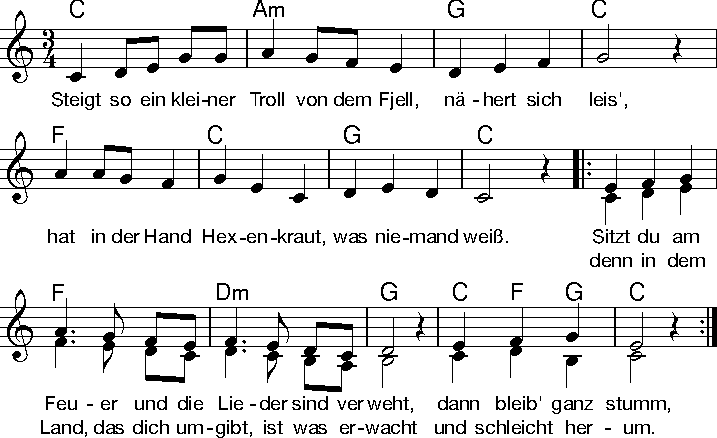
\includegraphics[draft=false, width=1\textwidth]{Noten/Lied016.pdf}	

\beginverse
\[C]Plötzlich in deinem \[Am]Nacken spürst du \[G]eiskalten \[C]Hauch,
\[F]Atem des Trolls \[C]trifft dich wie \[G]giftiger \[C]Rauch.
\endverse 

\beginchorus
Sitzt du am \[F]Feuer und die \[Dm]Lieder sind ver\[G]weht, \[C]dann \[F]bleib \[G]ganz \[C]stumm,
denn in dem \[F]Land, das dich um\[Dm]gibt, ist was er\[G]wacht \[C]und \[F]schleicht \[G]he\[C]rum.
\endchorus 

\beginverse
^Du führst den Becher ^Tee nun zum Mund. ^Was zauderst ^du?
^Blütenstaub im ^Zaubertrank ^raubt dir die ^Ruh'.
\endverse

\printchorus

\beginverse
^Wenn du in dieser ^Nacht deinen Schlaf ^findest nicht ^mehr,
^der kleine Troll ^macht uns're ^Träume so ^schwer.
\endverse


\printchorus

\endsong

\beginscripture{}
Der Autor (*1936), bekannt unter dem Fahrtennamen mac, verfasste viele bekannte Fahrtenlieder. Er beschäftigte sich intensiv mit skandinavischer Literatur und gab auch ein Jugendbuch mit dem Titel "Fjellwanderung" heraus.
\endscripture
